\section{Applications}

\subsection{Privacy-preserving pools}
\noindent Barring some exceptions, most blockchains allow public access to transaction details. These could include the source wallet, destination wallet, the tokens transferred, and other potentially sensitive information. Thus, traditional blockchain network innerworkings make privacy preservation nontrivial at the application layer. Fortunately, modern SNARKs can help address this issue when endowed with zero-knowledge properties. A prime example of this is Tornado Cash \cite{tornadocash}, an privacy-preserving pool running as a set of smart contracts on Ethereum network with some off-chain components. Tornado Cash allows one to deposit funds from wallet $A$, then withdraw the funds to a different wallet $B$. To do so, the user has to prove that they are the owner of the depositing wallet, and that they initiated it. They do so by constructing a commitment to the deposit using a secret value and the deposit details, and they submit this commitment to the smart contracts as part of the deposit process. The commitment is stored in a Merkle tree of all deposit commitments, and a nullifier is computed and stored to ensure the same deposit commitment is claimed only once. To withdraw, the user can do so via a different receiving wallet; they just need to submit a groth16 proof that their original commitment is present in the tree, which requires the source wallet info and secret they used to construct the commitment in the first place. The proof is just three group elements, as groth16 proofs usually are; but they encode way more information, like the merkle authentication path for the deposit commitment the tree, and the correct hashing procedure to produce the commitment and nullifier.\\

\begin{figure}[ht]
\centering
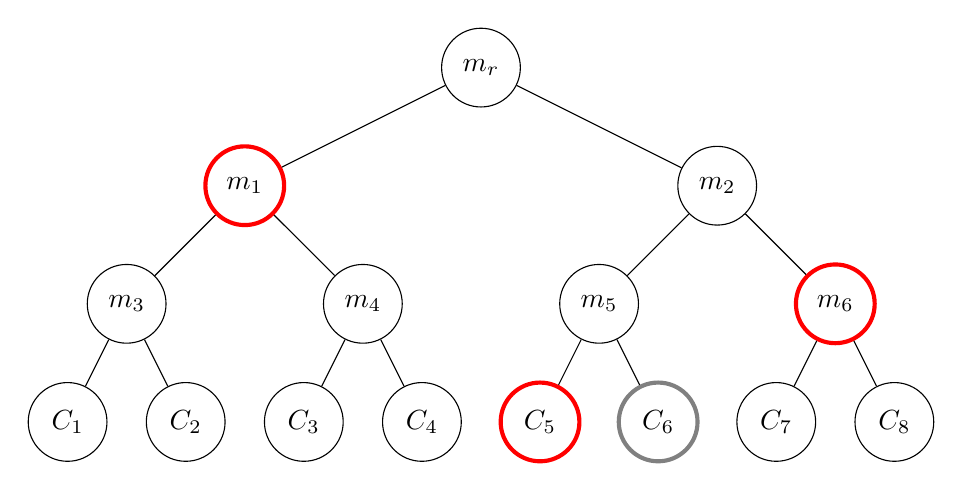
\begin{tikzpicture}[
    level 1/.style={sibling distance=60mm},
    level 2/.style={sibling distance=30mm},
    level 3/.style={sibling distance=15mm},
    every node/.style={draw, circle, minimum size=10mm}
]
    % Root node
    \node {$m_r$}
        % Level 1
        child {node[draw=red, line width=1.5pt] {$m_1$}
            % Level 2
            child {node {$m_3$}
                % Level 3
                child {node {$C_1$}}
                child {node {$C_2$}}
            }
            child {node {$m_4$}
                % Level 3
                child {node {$C_3$}}
                child {node {$C_4$}}
            }
        }
        child {node {$m_2$}
            % Level 2
            child {node {$m_5$}
                % Level 3
                child {node[draw=red, line width=1.5pt] {$C_5$}}
                child {node[draw=gray, line width=1.5pt] {$C_6$}}
            }
            child {node[draw=red, line width=1.5pt] {$m_6$}
                % Level 3
                child {node {$C_7$}}
                child {node {$C_8$}}
            }
        };
\end{tikzpicture}
    \caption{Merkle tree with authentication path (in red) for commitment C6 (in gray)}
\label{fig:merkle-tree}
\end{figure}

\noindent For instance, if we make a deposit (commitment $C_6$ in figure \ref{fig:merkle-tree}) and we want to withdraw later, we would submit a proof $\pi$ encoding the secret, the nullifier hash, other commitment hash inputs, and the list of nodes and their relative positions in the hashing sequence that would lead to the correct root if $C_6$ were in fact within the tree. The tornado cash infrastructure includes off-chain components with this functionality. In particular, it contains circuits written in Circom which can be used to generate and verify groth16 proofs of deposit commitment validity, and front-end/command-line tools to generate proofs.

\subsection{Privacy-preserving blockchains}
\noindent Beneath the application layer there are blockchains utilizing zero-knowledge properties of SNARKs for infrastructural privacy preservation. For each transaction submitted, such systems must obscure the source, relevant currencies, amounts used, and payment recipients. Zerocash \cite{zcash} is a notable example of a network that does such a thing. Intended to be a privacy-preserving version of Bitcoin \cite{bitcoin}, Somewhat similar to (and preceding) Tornado Cash, Zerocash the unspent-transaction-output (UTXO) model, where transactions create so-called ``unspent funds'' that the party who ``owns'' them is entitled to spend. When they do spend those funds, another record of ``unspent funds'' for the recipient of the spending is created. These UTXO records are stored in a merkle tree, and spending funds requires proving knowledge of a leaf in the tree corresponding to the funds. Early versions of Zerocash used groth16 for this, but the NU5 upgrade of 2022 switched to the universal halo2 proof system \cite{halo2}, which enables a combination of a PlonK-style arithmetization and commitment scheme requiring no trusted setup (and adding flexibility for more complex future privacy-preserving computation).

\subsection{Verifiable Virtual Machines (VVM)}
\noindent So-called ``Zero-knowledge virtual machines'' (zkVMs) have emerged as an elegant solution to settling transaction batches from layer 2 (L2) blockchains on the layer 1 (L1) chain they derive crypto-economic security from. We use the more accurate phrase ``verifiable virtual machine'' (VVM) since succinctness is a higher priority than zero-knowledge in most L2 architectures. To align with real-world use cases like polygon zkEVM, Scroll, and others, we consider a centralized L2 blockchain with a single node that receives transactions, orders them, and creates blocks from them. The node then constructs a SNARK of block validity and sends this proof to a verifier contract on the L1 chain for verification. The SNARK is constructed from a large circuit which must constrain the witness to describe only valid computation paths through the VVM. Since the computation structure can change every time, this calls for universal SNARKs, of which PlonK and its variants are popular choices. More concretely, many VVM implementations use circuit domain-specific languages (DSLs) like halo2 to implement the circuits constraining the computation details.\\

\noindent A crucial point of consideration here is that not all computations performed in VVMs are ``SNARK-friendly''; a prime example of this is hash functions like SHA256 which use non-linear or non-algebraic operations like bit mixing. This can cause the circuits constraining this computation to be overly complex and inefficient. To meet this end, lookup-based methods are of great interest here since they can avoid constraining ``SNARK-unfriendly'' operations directly without losing soundness. An example of this is lies in the proof for validity of transaction that called a contract function using \texttt{sha256()}. Instead of constraining the exact sha-256 computation, the prover and verifier would agree on a publicly known table of acceptable inputs and outputs for SHA-256, which the prover commits to as part of the proof. The verifier does not need to know the whole table - they just need to know a commitment to the one considered correct. This can then be compared with what the prover committed to.\\
